\documentclass{anstrans}
%%%%%%%%%%%%%%%%%%%%%%%%%%%%%%%%%%%
\title{Load Balancing for Massively Parallel Transport Sweeps on Unstructured Meshes }
\author{Tarek H. Ghaddar,$^{*}$ Jean C. Ragusa$^{*}$}

\institute{
$^{*}$Dept. of Nuclear Engineerin, Texas A\&M University, Animal Industries Engineering Building, College Station, TX, 77843-3133
\and

}

\email{tghaddar@tamu.edu \and jean.ragusa@tamu.edu}

% Optional disclaimer: remove this command to hide
\disclaimer{Notice: this manuscript is a work of fiction. Any resemblance to
actual articles, living or dead, is purely coincidental.}

%%%% packages and definitions (optional)
\usepackage{graphicx} % allows inclusion of graphics
\usepackage{booktabs} % nice rules (thick lines) for tables
\usepackage{microtype} % improves typography for PDF
%Math Symbols
\newcommand{\vr}{\vec{r}}
\newcommand{\vo}{\vec{\Omega}}
%Allows [H] option
\usepackage{float}
%Allow page breaks within align
\allowdisplaybreaks
%Allows for easy pseudocode.
\usepackage{listings}
%Changing spacing in itemized lists
\usepackage{enumitem}
\setlist{nosep}
%Include a pdf file
\usepackage{pdfpages}
%Eps figures
\usepackage{epstopdf}
%Algorithm
\usepackage{algorithm}
\usepackage{algorithmic}

\newcommand{\SN}{S$_N$}
\renewcommand{\vec}[1]{\bm{#1}} %vector is bold italic
\newcommand{\vd}{\bm{\cdot}} % slightly bold vector dot
\newcommand{\grad}{\vec{\nabla}} % gradient
\newcommand{\ud}{\mathop{}\!\mathrm{d}} % upright derivative symbol

\begin{document}
%%%%%%%%%%%%%%%%%%%%%%%%%%%%%%%%%%%%%%%%%%%%%%%%%%%%%%%%%%%%%%%%%%%%%%%%%%%%%%%%
\section{Introduction}
\label{ch:introduction}
When running any massively parallel code, load balancing is a priority in order to achieve the best possible parallel efficiency. A load balanced problem has an equal number of degrees of freedom per processor. Load balancing is important in order to minimize idle time for all processors by equally distributing (as much as possible) the work each processor has to do.

The concepts and results presented in this thesis are used by PDT, Texas A\&M University's massively parallel deterministic transport code. It is capable of multi-group simulations and employs discrete ordinates for angular discretization. PDT features steady-state, time-dependent, criticality, and depletion simulations. It solves the transport equation for neutron, thermal, gamma, coupled neutron-gamma, electron, and coupled electron-photon radiation. PDT  has been shown to scale on logically Cartesian grids out to 750,000 cores. Logically Cartesian grids contain regular convex grid units that allow for vertex motion inside them, in order to conform to curved shapes. 

The following are the completed goals of this thesis:
\begin{itemize}
\item Implement unstructured meshing capability in PDT for 2D and 2D extruded problems.
\item Generate unstructured mesh in parallel using the same partitioning scheme and number of processors as the Cartesian-grid transport sweep.
\item {Perform stitching between meshed subdomains to preserve interface continuity.}
\item Implement load balancing algorithms for unstructured meshes in PDT. A load balanced problem is determined by the value of $f$, where $f$ is the subset with the maximum number of cells, divided by the average number of cells per subset. A perfectly balanced problem has $f = 1$.
\item Verify and test code to prove load balancing algorithm effectiveness, in addition to unstructured meshing capability. 
\item Show results of the parallel transport sweeps on unstructured meshes for benchmark problems.
\end{itemize}

The unstructured meshing capability being added into PDT was of paramount importance because it allows the user to define the problem geometry without having to conform the mesh to the problem geometry. The need to move vertices within convex grids is no longer needed, so the user only needs to define the geometry of the problem. A 2D unstructured mesh is created utilizing the Triangle mesh generator. The resulting mesh can be extruded in the third spatial dimension. The 2D extruded grid is not as generic as a fully tetrahedral grid (such implementation is left as future work). 

%%%%%%%%%%%%%%%%%%%%%%%%%%%%%%%%%%%%%%%%%%%%%%%%%%%%%%%%%%%%%%%%%%%%%%%%%%%%%%%%


%%%%%%%%%%%%%%%%%%%%%%%%%%%%%%%%%%%%%%%%%%%%%%%%%%%%%%%%%%%%%%%%%%%%%%%%%%%%%%%%
\section{Motivation and Methods}
\label{ch:motivation}

The capability for PDT to generate and run on an unstructured mesh is important because it allows us to run problems without having to conform our mesh to the problem as much. The idea is to have a logically Cartesian grid (creating orthogonal ``subsets") with an unstructured mesh inside each subset. These logically Cartesian subdomains are obtained using cut planes in 3D and cut lines in 2D. Figure \ref{grid} demonstrates this functionality. It is decomposed into 3 subsets in x and 3 in y, with the first two subsets meshed using the Triangle Mesh Generator\cite{triangle}, a 2D mesh generator.

\begin{figure}[H]
\centering
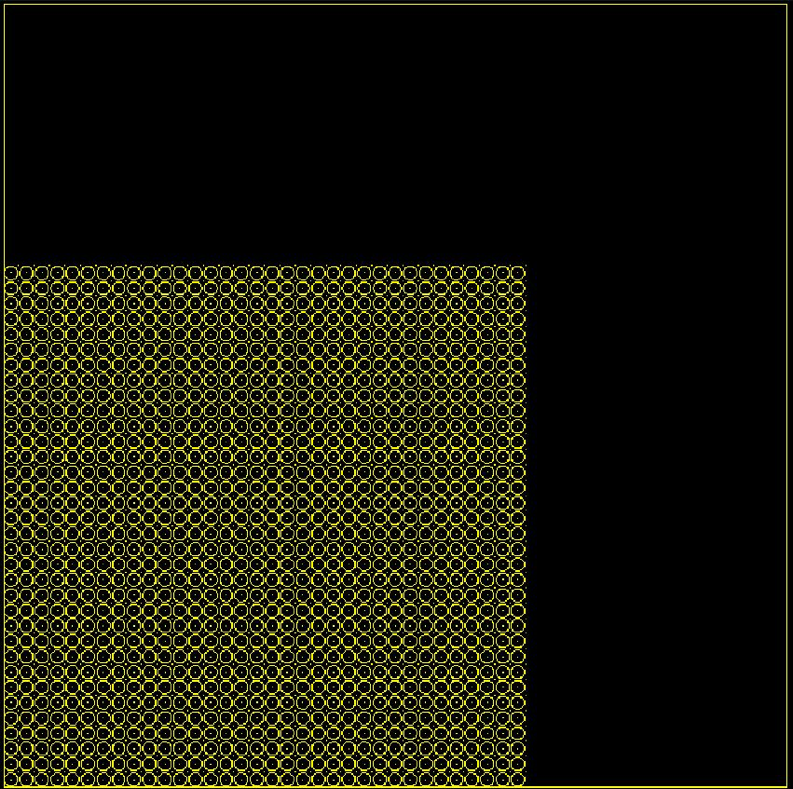
\includegraphics[scale = 0.45]{figures/lattice.png}
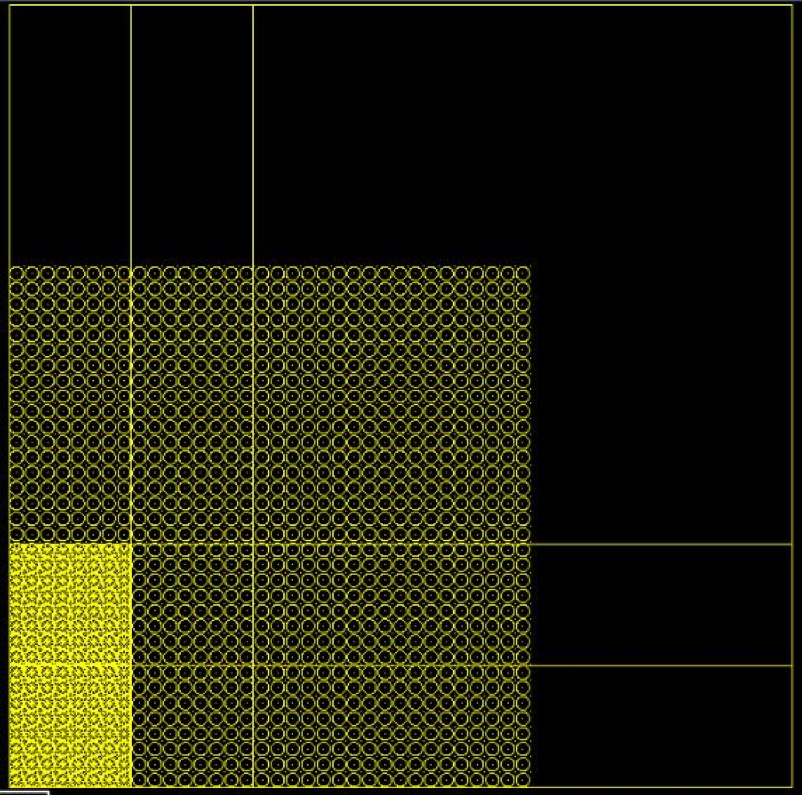
\includegraphics[scale = 0.45]{figures/subsetlattice.png}
\caption{A PSLG describing a fuel lattice, and with an orthogonal ``subset" grid imposed on the PSLG.}
\label{grid}
\end{figure}

This orthogonal grid is superimposed and each subset is meshed in parallel.  Subsets are now the base structured unit when calculating our parallel efficiency. Discontinuities along the boundary are fixed by ``stitching'' hanging nodes, creating degenerate polygons along subset boundaries. Because PDT's spatial discretization employs Piece-Wise Linear Discontinuous (PWLD) finite element basis functions, there is no problem solving on degenerate polygons. 

When using the unstructured meshing capability in PDT, the input geometry is described by a Planar Straight Line Graph (PSLG). After superimposing the orthogonal grid, a PSLG is created for each subset, and meshed. Because the input's and each subset's PSLG must be described and meshed in 2D, the mesh can be extruded in the $z$ dimension in order to give us the capability to run on 3D problems. Obviously, this is not as good as an unstructured tetrahedral mesh, but for many problems, it is a great capability to have. 


\section{The Load Balancing Algorithm}

When discussing the parallel scaling of transport sweeps, a load balanced problem is of great importance. A load balanced problem has an equal number of degrees of freedom per processor. Load balancing is important in order to minimize idle time for all processors by equally distributing (as much as possible) the work each processor has to do.  For the purposes of unstructured meshes in PDT, we are looking to ``balance'' the number of cells. Ideally, each processor will be responsible for an equal number of cells. 

If the number of cells in each subset can be reasonably balanced, then the problem is effectively load balanced. The Load Balance algorithm described below details how the subsets will be load balanced. In summary, the procedure of the algorithm involves moving the initially user specified $x$ and $y$ cut planes, re-meshing, and iterating until a reasonably load balanced problem is obtained.  Equation \ref{metric_def} shows the equation for calculating the load balancing metric, which dictates how balanced or unbalanced the problem is.
\begin{equation}
f =\frac{\underset{ij}{\text{max}}(N_{ij})}{\frac{N_{tot}}{I\cdot J}},
\label{metric_def}
\end{equation}
where $f$ is the load balance metric, $N_{ij}$ is the number of cells in subset $i,j$, $N_{tot}$ is the global number of cells in the problem, and $I$ and $J$ are the total number of in the $x$ and $y$ direction, respectively. The metric is a measure of the maximum number of cells per subset divided by the average number of cells per subset.

The load balancing algorithm moves cut planes based on two sub-metrics, $f_I$ and $f_J$. Equation ~\eqref{submetric} defines these two parameters:
\begin{align}
f_I &= \underset{i}{\text{max}}[\sum_{j} N_{ij}]/\frac{N_{tot}}{I} \notag \\
f_J &= \underset{j}{\text{max}}[\sum_{i} N_{ij}]/\frac{N_{tot}}{J}.
\label{submetric}
\end{align}

$f_I$ is calculated by taking the maximum number of cells per column and dividing it by the average number of cells per column. $f_j$ is calculated by taking the maximum number of cells per row and dividing it by the average number of cells per row. If these two numbers are greater than predefined tolerances, the cut lines in the respective directions are redistributed. Once redistribution and remeshing occur, a new metric is calculated. This iterative process occurs until a maximum number of iterations is reached, or until $f$ converges within the user defined tolerance. The Load Balance algorithm behaves as follows:

\lstinputlisting[language = C++, basicstyle = \footnotesize]{loadbalance.cc}

\begin{algorithm}
\textbf{Redistribute:} A function that moves cut lines in either X or Y. \\
\begin{algorithmic}
\STATE \textbf{Input:}CutLines (X or Y vector that stores cut lines). 
\STATE \textbf{Input:} num\_tri\_row or num\_tri\_col, a pArray containing number of triangles in each row or column 
\STATE \textbf{Input:} The total number of triangles in the domain, $N_{tot}$
\STATE stapl::array\_view num\_tri\_view, over num\_tri\_row/column
\STATE stapl::array\_vew offset\_view
\STATE stapl::partial\_sum(num\_tri\_view) \COMMENT {Perform prefix sum}
\COMMENT {We now have a cumulative distribution stored in offset\_view}
\FOR {$i = 1$ :CutLines.size()-1}

	\STATE vector $<$double$>$ pt1 = [CutLines(i-1), offset\_view(i-1)]
	\STATE vector $<$double$>$ pt2 = [CutLines(i), offset\_view(i)]
	\STATE ideal\_value = $i\cdot \frac{N_{tot}}{\text{CutLines.size()}-1}$
	\STATE X-intersect(pt1,pt2,ideal\_value) \COMMENT{Calculates the X-intersect of the line formed by pt1 and pt2 and the line y = ideal\_value.}
	\STATE CutLines(i) = X-intersect
\ENDFOR
\end{algorithmic}
\end{algorithm}



%%%%%%%%%%%%%%%%%%%%%%%%%%%%%%%%%%%%%%%%%%%%%%%%%%%%%%%%%%%%%%%%%%%%%%%%
\section{Results}
\label{ch:results}
The following sections will showcase the metric behavior and convergence for three test cases and the new unstructured meshing capability both in 2D and 3D.

\subsection{Test Cases for Metric Behavior and Convergence}
\label{sec:convergence}
In order to showcase the behavior of the load balancing metric, calculated by Eq. \ref{metric_def} three test cases are presented. Figure \ref{opp} shows the first test case, a 20 cm by 20 cm domain with two pins in opposite corners of the domain. Figure \ref{same} shows the same size domain but with the pins on the same side.These are two theoretically very unbalanced cases, as geometrically there are two features located distantly from each other with an empty geometry throughout the rest of the domain. Figure \ref{lattice} shows a lattice and reflector, which due to it's denser and repeated geometry, theoretically is a more balanced problem. 

A series of 162 inputs was constructed for each case. These inputs are constructed by varying the maximum triangle area from the coarsest possible to 0.01 cm\textsuperscript{2} and the number of subsets, $N$ from 2$\times$2 to 10$\times$10. 

\begin{figure}[H]
\centering
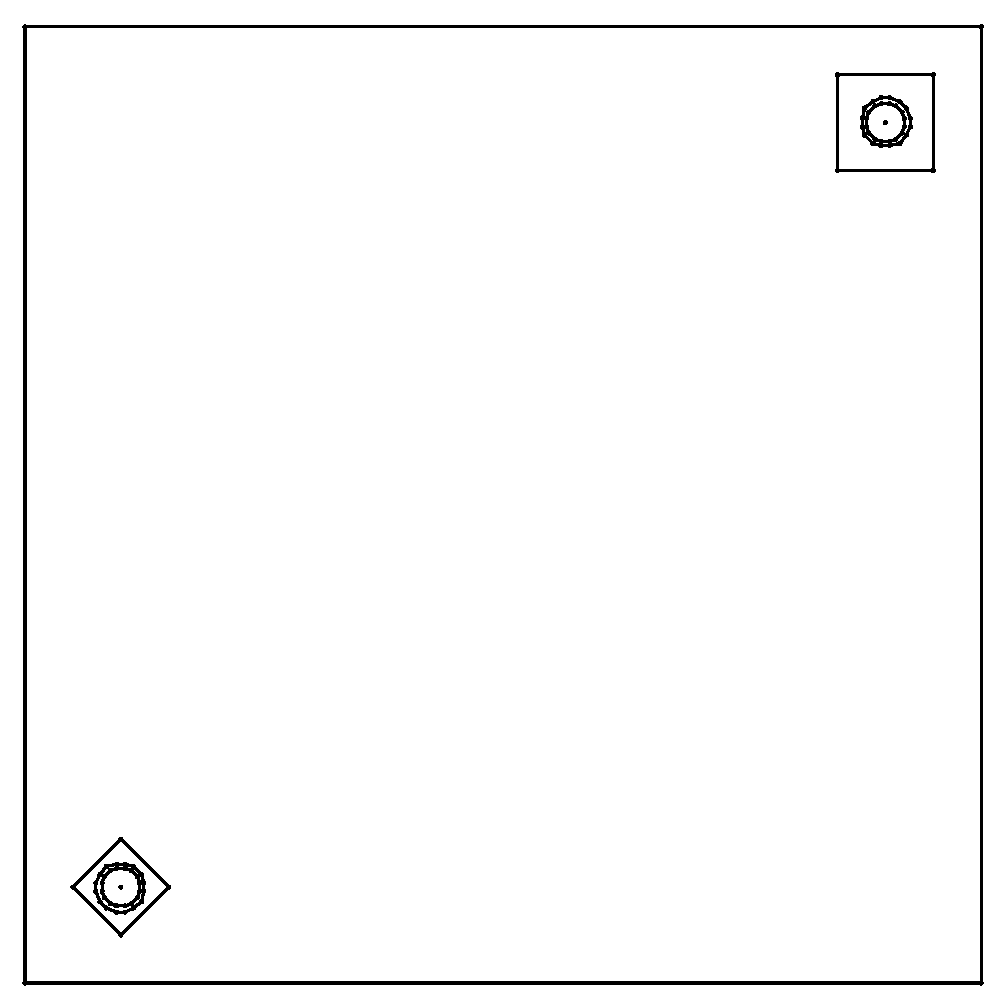
\includegraphics[scale = 0.5]{figures/unbalanced_lattice.eps}
\caption{The first test case used in order to test effectiveness and convergence of the load balancing metric.}
\label{opp}
\end{figure}

\begin{figure}[H]
\centering
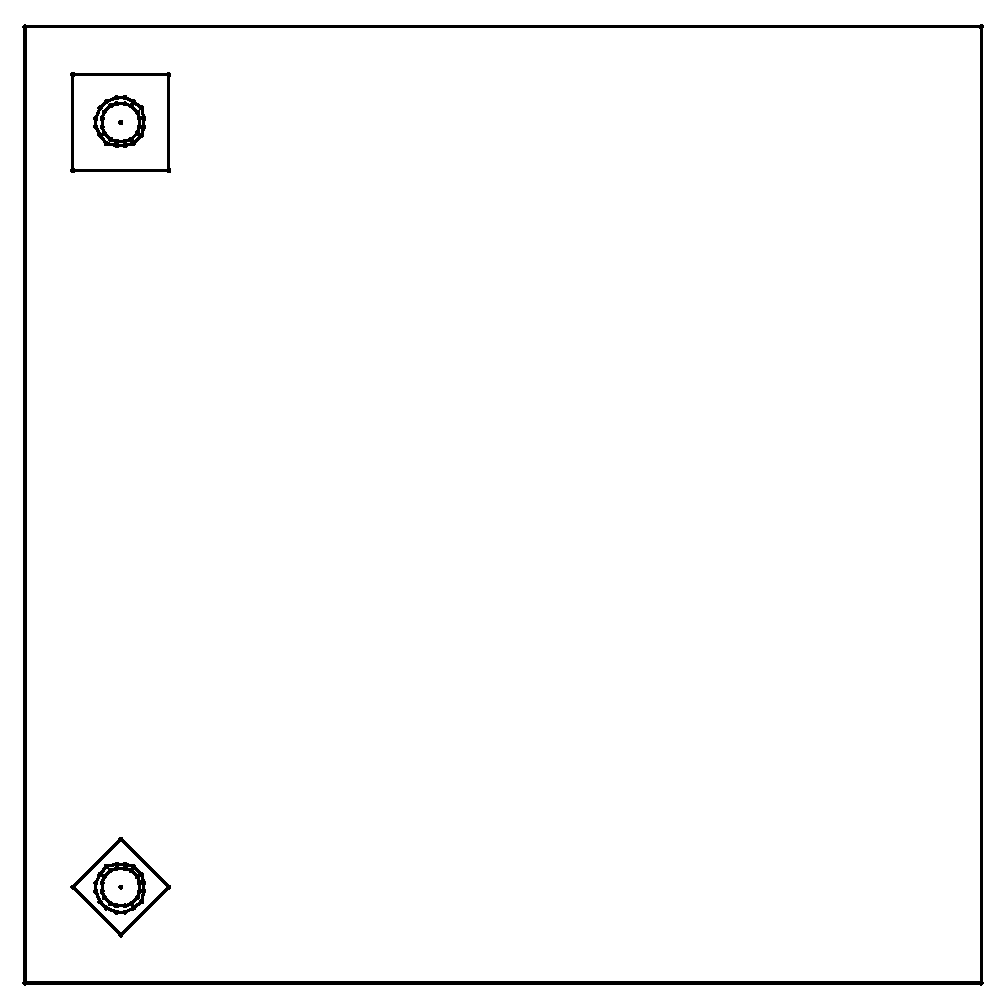
\includegraphics[scale = 0.5]{figures/unbalanced_pins_same_side.eps}
\caption{The second test case used in order to test effectiveness and convergence of the load balancing metric.}
\label{same}
\end{figure}

\begin{figure}[H]
\centering
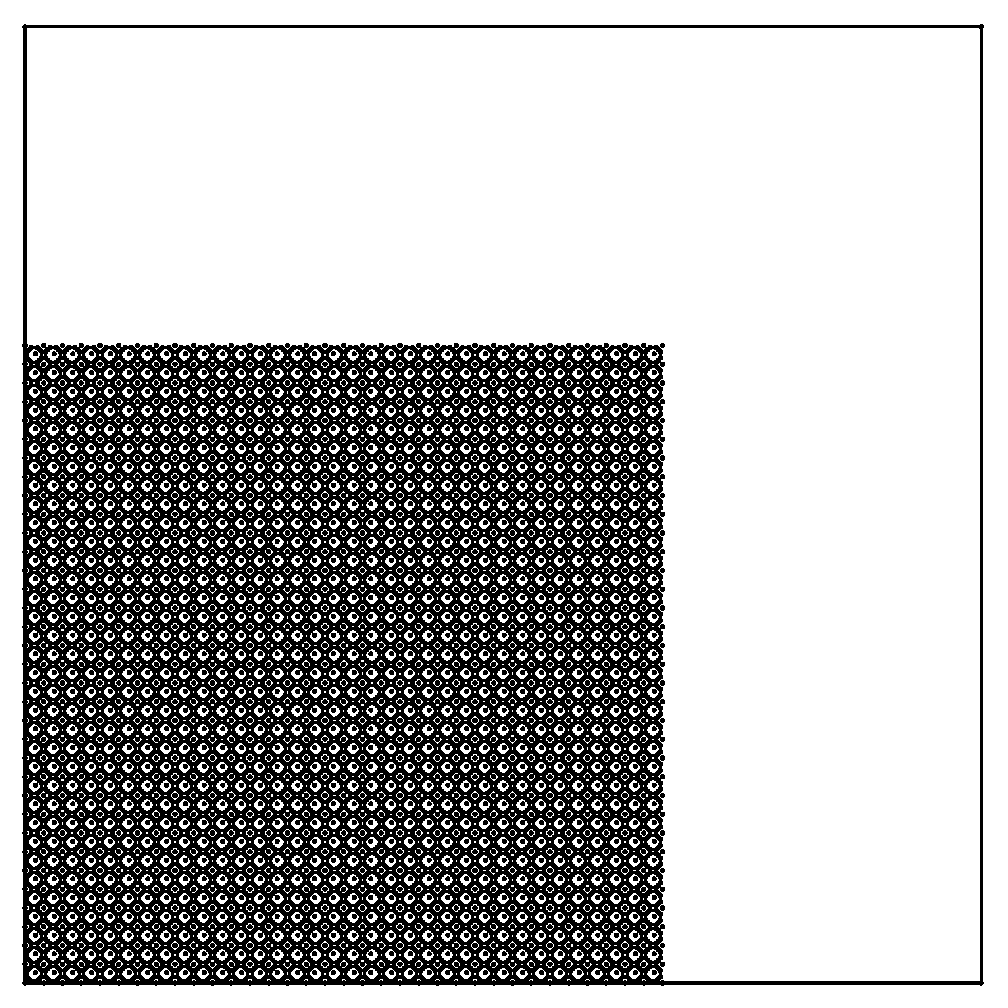
\includegraphics[scale = 0.5]{figures/lattice-12-shifted.eps}
\caption{The third test case used in order to test effectiveness and convergence of the load balancing metric.}
\label{lattice}
\end{figure}

\subsection{Metric Behavior and Convergence}

For each test case, the 162 input inputs are run twice, once with no load balancing iterations, and once with ten load balancing iterations. The best metric is reported and recorded. Three figures for each test cases are presented below: the first figure will show the metric behavior for no iterations, the second figure will show the metric behavior for each input run with ten load balancing iterations, and the third figure will show a ratio of the ten iteration runs over the no iteration runs.

Figure \ref{oppnoiter} shows the metric behavior for Fig. \ref{opp}. The maximum metric value is 24.7650, and occurs when Fig. \ref{opp} is run with 8x8 subsets and a maximum triangle area of 1.6 cm\textsuperscript{2}. The minimum metric value is 1.0016 and occurs when Fig. \ref{opp} is run with 4x4 subsets and a maximum triangle area of 0.04 cm\textsuperscript{2}. 

\begin{figure}[H]
\centering
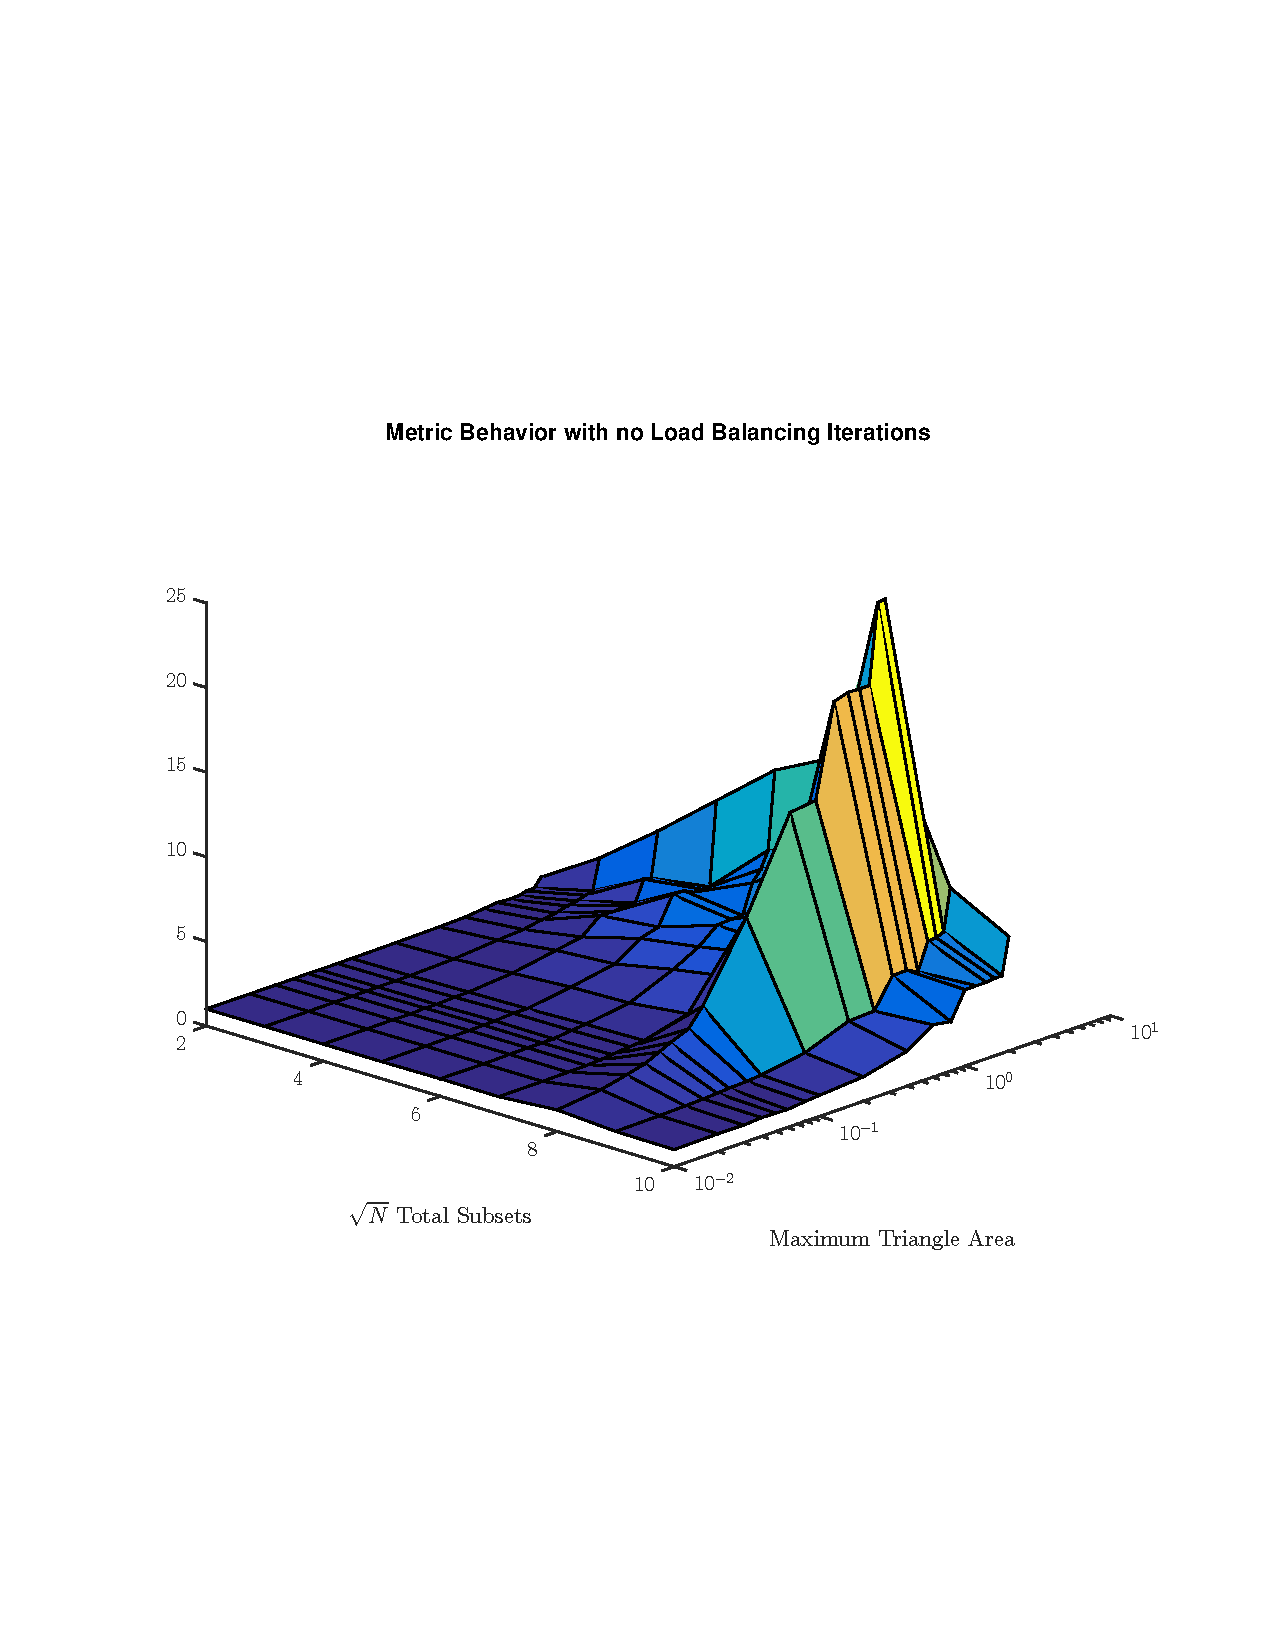
\includegraphics[scale=0.5, trim = 0cm 8cm 0cm 7cm,clip]{figures/OppNoIter.pdf}
\caption{The metric behavior of the first test case run with no load balancing iterations.}
\label{oppnoiter}
\end{figure}

Figure \ref{oppiter} shows the metric behavior for Fig. \ref{opp} after 10 load balancing iterations. The maximum metric value is 5.0538 and occurs when Fig. \ref{opp} is run with 10x10 subsets and a maximum triangle area of 1.2 cm\textsuperscript{2}. The minimum metric value is 1.0017 and occurs when Fig. \ref{opp} is run with 4x4 subsets and a maximum triangle area of 0.04 cm\textsuperscript{2}.

\begin{figure}[H]
\centering
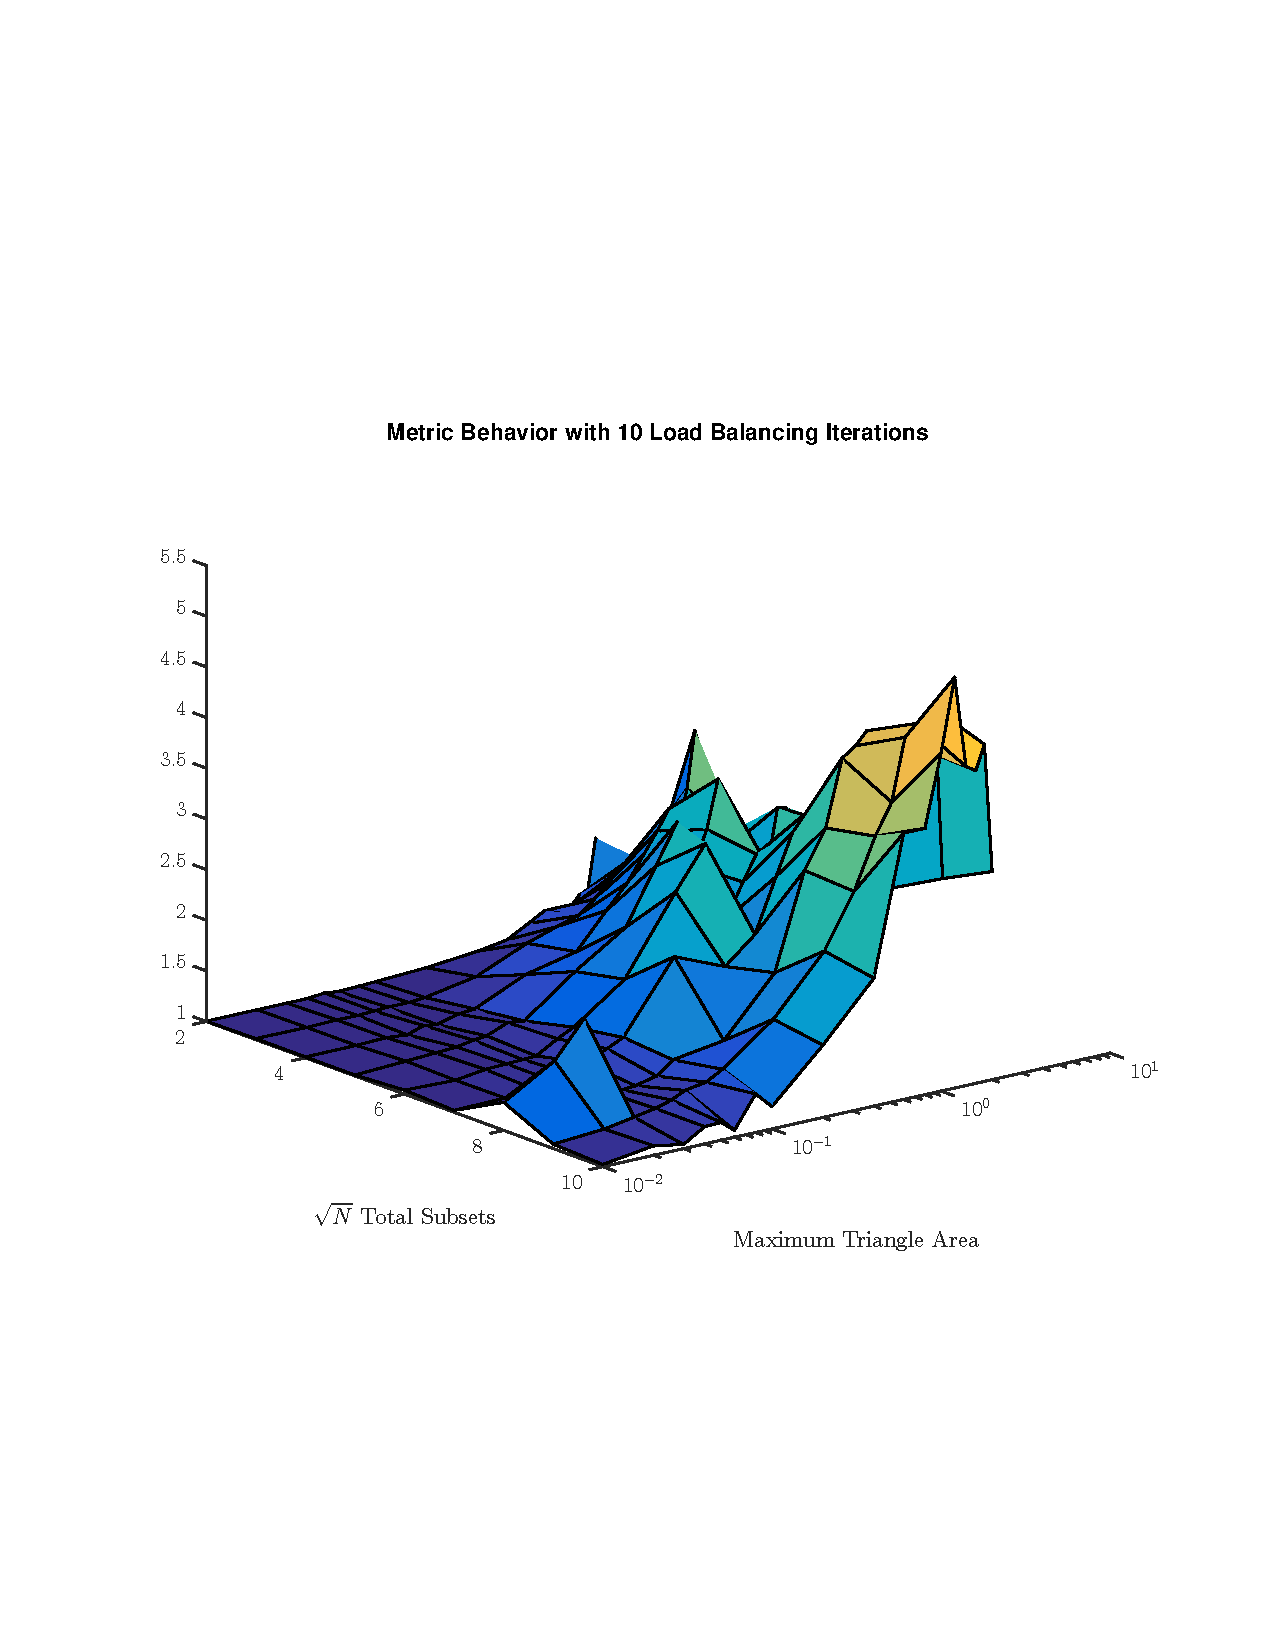
\includegraphics[scale=0.5, , trim = 2cm 6cm 2cm 7cm,clip]{figures/OppIter.pdf}
\caption{The metric behavior of the first test case run with 10 load balancing iterations.}
\label{oppiter}
\end{figure}

Figure \ref{oppdiff} shows the difference in metric behavior for Fig. \ref{opp}. This difference is calculated by dividing the metric with no iterations by the metric with 10 iterations. The maximum improvement has a value of 0.1097 and occurs for Fig. \ref{opp} is run with 8x8 subsets with a maximum triangle area of 1.6 cm\textsuperscript{2}. The minimum improvement has a value of very close to 1.0 and occurs for many of the inputs. 

\begin{figure}[H]
\centering
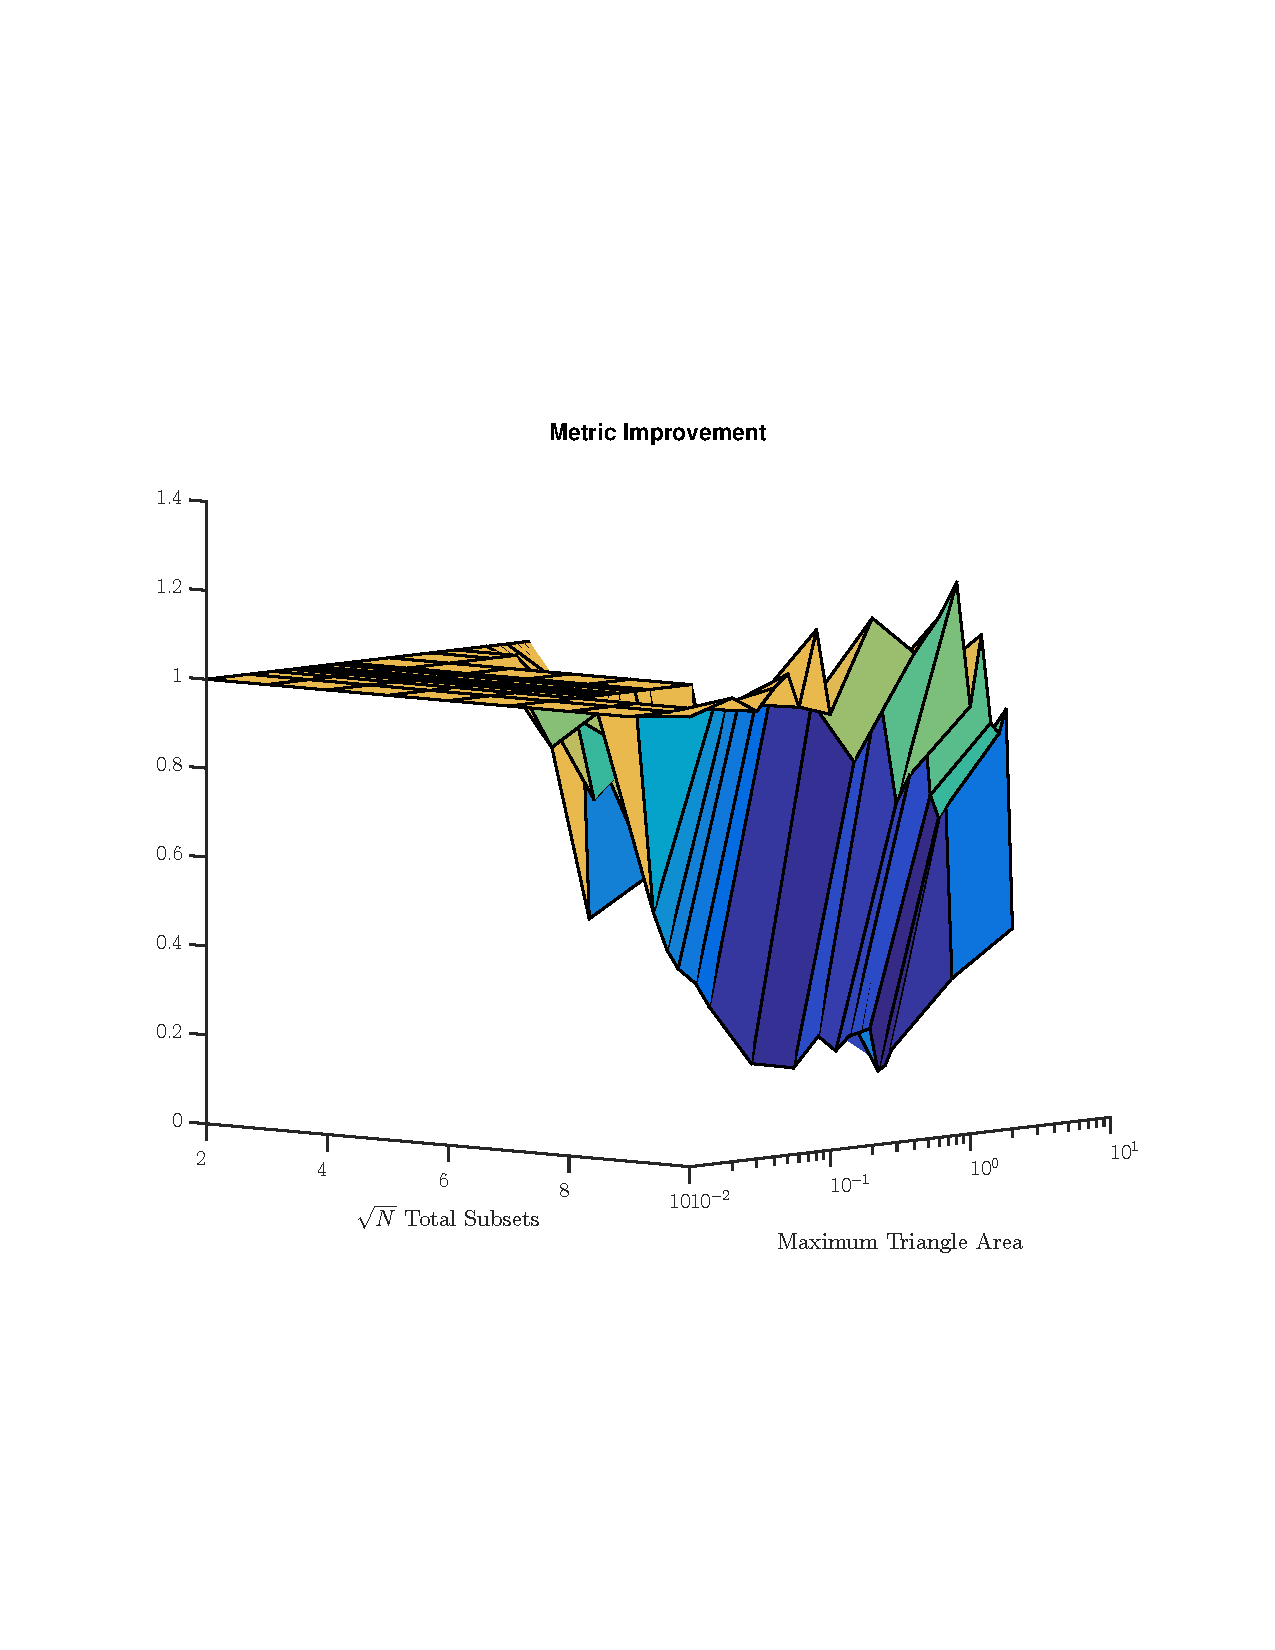
\includegraphics[scale=0.5, trim = 2cm 6cm 2cm 7cm,clip]{figures/OppDiff.pdf}
\caption{The difference in metric behavior between no iteration and 10 iterations. The closer the z-value to zero, the better the improvement.}
\label{oppdiff}
\end{figure}

Figure \ref{samenoiter} shows the metric behavior for Fig. \ref{same}. The maximum metric is 22.6654 and occurs when Fig. \ref{same} is run with 8x8 subsets with a maximum triangle area of 1.8 cm\textsuperscript{2}. The minimum metric is 1.0024 and occurs when Fig. \ref{same} is run with 2x2 subsets with a maximum triangle are of 0.01 cm\textsuperscript{2}.

\begin{figure}[H]
\centering
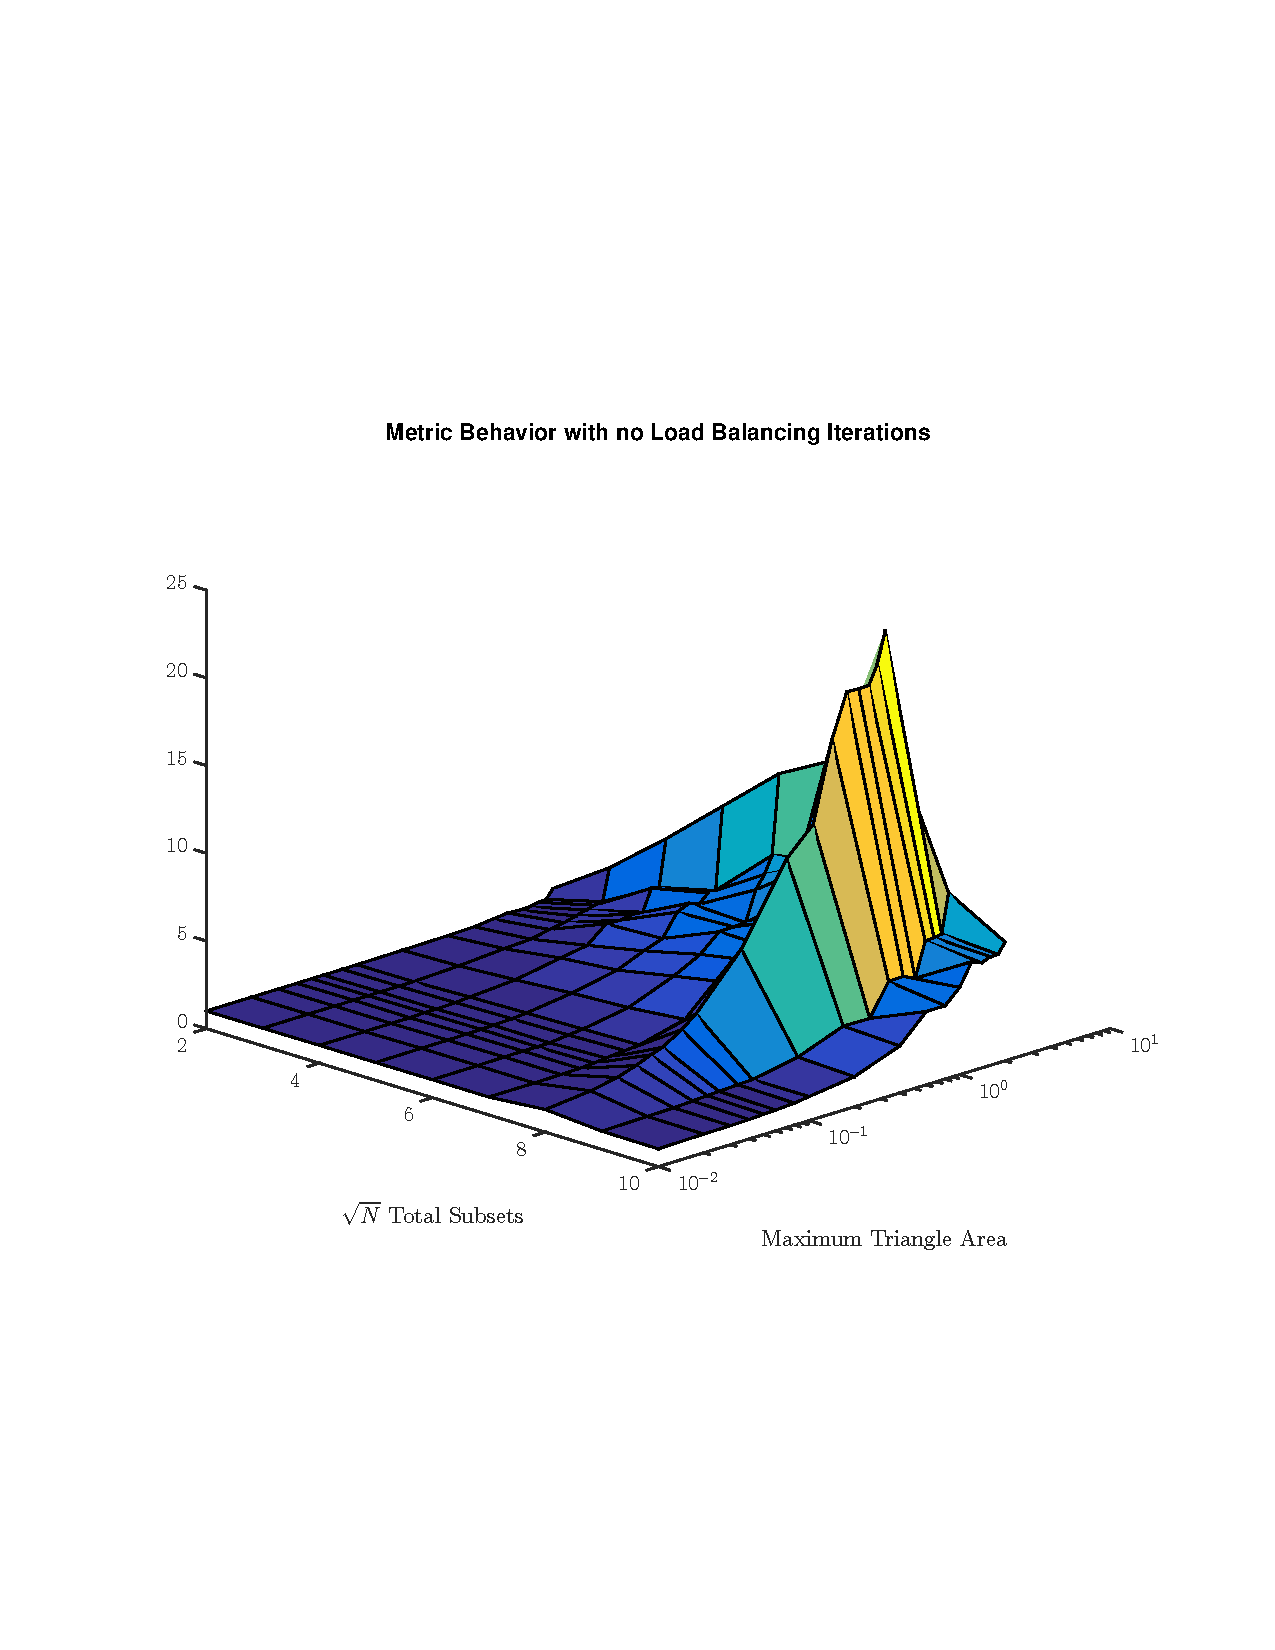
\includegraphics[scale=0.5, trim = 2cm 6cm 2cm 7cm,clip]{figures/SameNoIter.pdf}
\caption{The metric behavior of the second test case run with no load balancing iterations.}
\label{samenoiter}
\end{figure}

Figure \ref{sameiter} shows the metric behavior for Fig. \ref{same} after ten load balancing iterations. The maximum metric is 3.9929 and occurs when Fig. \ref{same} is run with 10x10 subsets with a maximum triangle area of 1.8 cm\textsuperscript{2}. The minimum metric is 1.0024 and occurs when Fig. \ref{same} is run with 2x2 subsets with a maximum triangle are of 0.01 cm\textsuperscript{2}.

\begin{figure}[H]
\centering
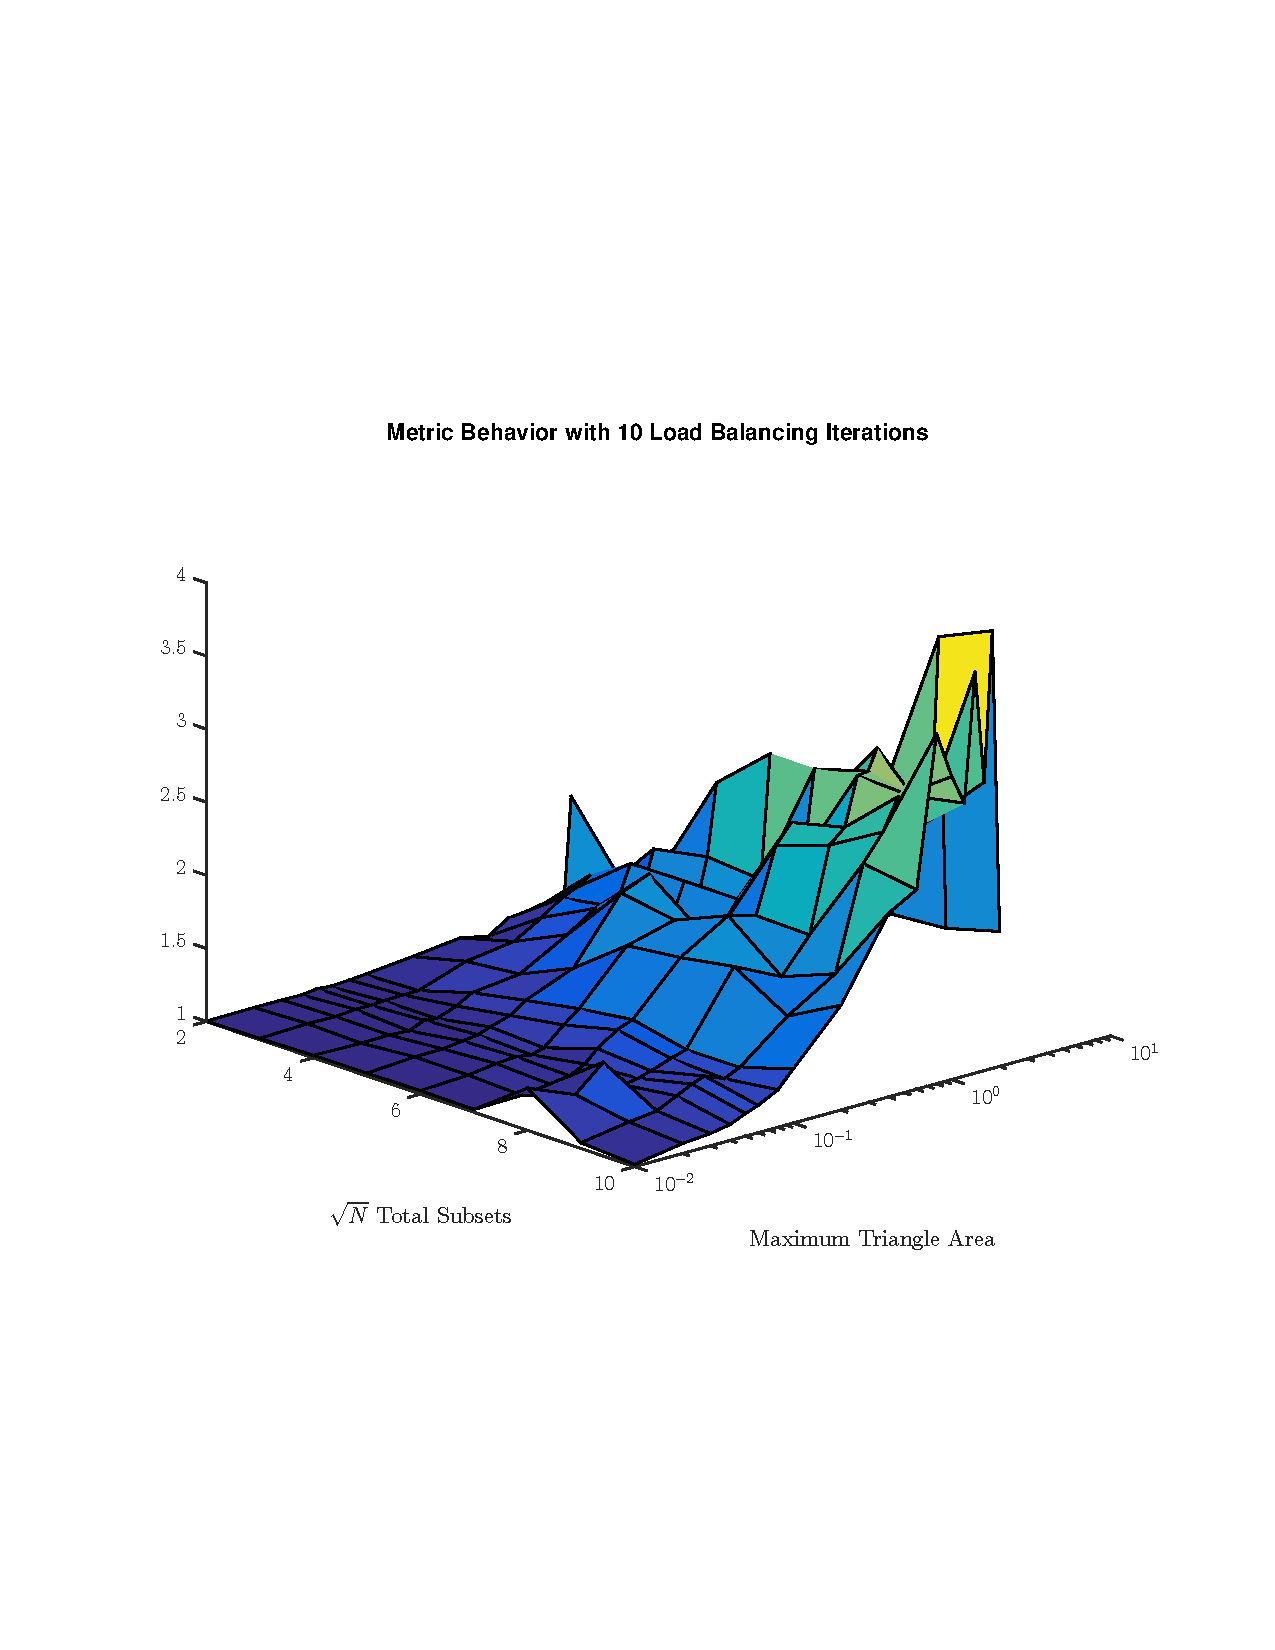
\includegraphics[scale=0.50, trim = 2cm 6cm 2cm 7cm,clip]{figures/SameIter.pdf}
\caption{The metric behavior of the second test case run with 10 load balancing iterations.}
\label{sameiter}
\end{figure}

Figure \ref{samediff} shows the difference in metric behavior for Fig. \ref{same}. The maximum improvement has a value of 0.1090 and occurs for Fig. \ref{same} is run with 8x8 subsets with Triangle's coarsest possible mesh generation settings. The minimum improvement has a value of very close to 1.0 and occurs for many of the inputs. 

\begin{figure}[H]
\centering
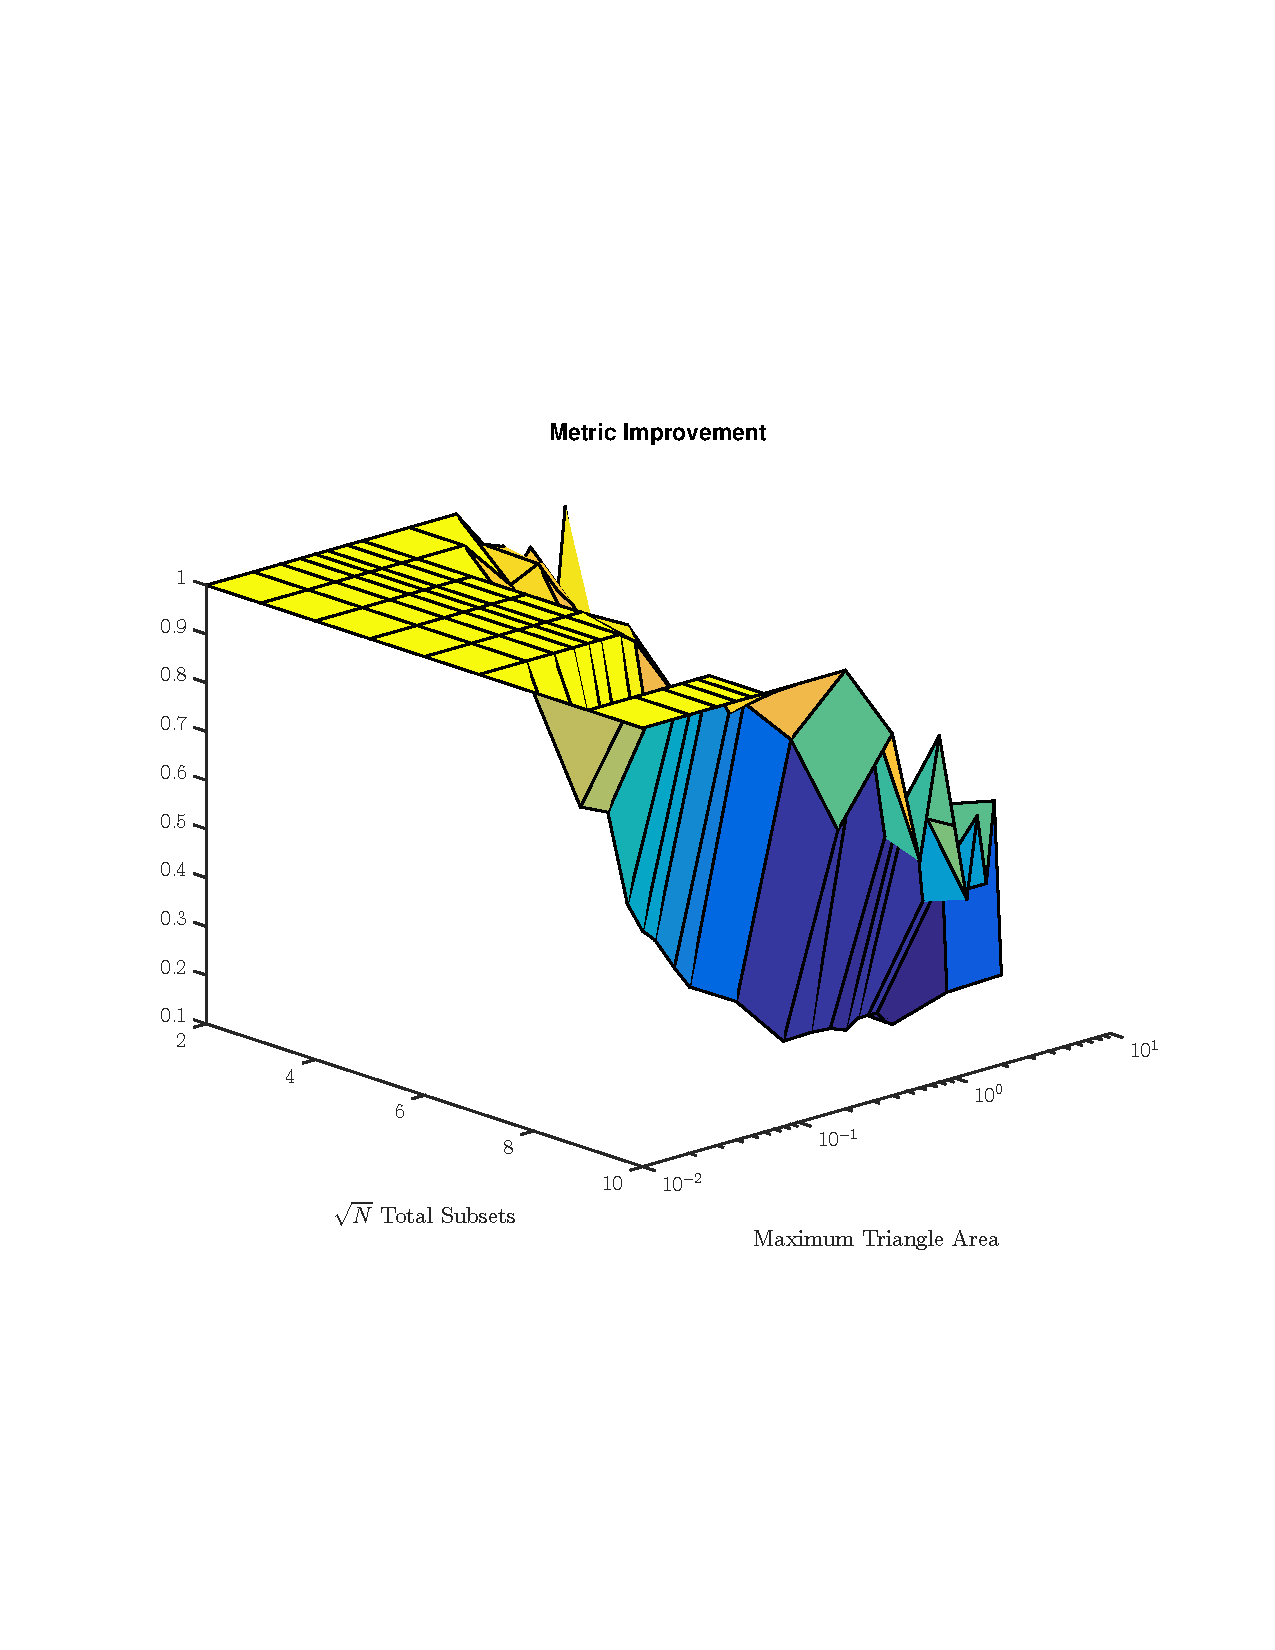
\includegraphics[scale=0.50, trim = 2cm 6cm 2cm 7cm,clip]{figures/SameDiff.pdf}
\caption{The difference in metric behavior of the second test case with no iteration and 10 iterations. The closer the z-value to zero, the better the improvement.}
\label{samediff}
\end{figure}

Figure \ref{latticenoiter} shows the metric behavior for Fig. \ref{lattice}. The maximum metric is 2.6489 and occurs when Fig. \ref{lattice} is run with 10x10 subsets with a maximum triangle area of 1.8 cm\textsuperscript{2}. The minimum metric is 1.0179 and occurs when Fig. \ref{lattice} is run with 2x2 subsets with a maximum triangle are of 0.08 cm\textsuperscript{2}.

\begin{figure}[H]
\centering
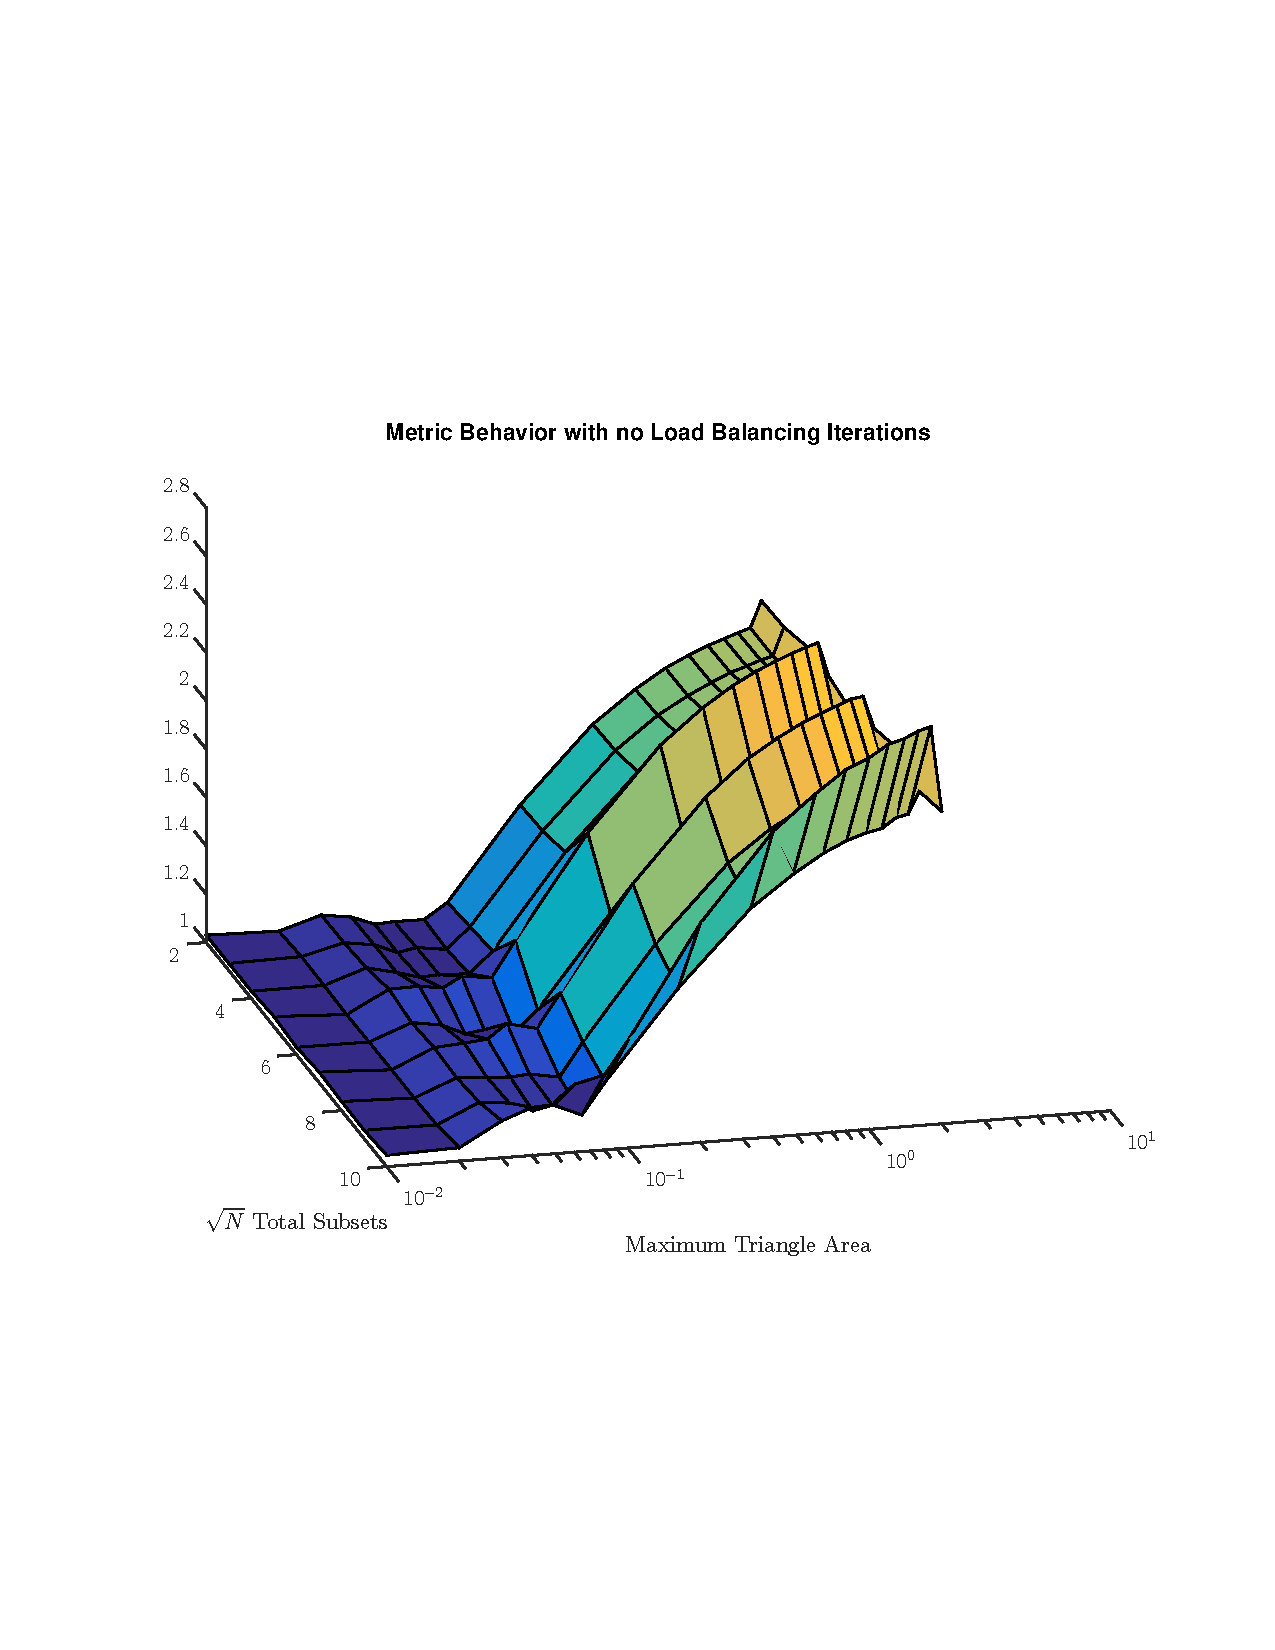
\includegraphics[scale=0.50, trim = 2cm 6cm 2cm 7cm,clip]{figures/lattice_no_iter.pdf}
\caption{The difference in metric behavior of the third test case with no load balancing iterations.}
\label{latticenoiter}
\end{figure}

Figure \ref{latticeiter} shows the metric behavior for Fig. \ref{lattice} after ten load balancing iterations. The maximum metric is 2.2660 and occurs when Fig. \ref{lattice} is run with 10x10 subsets with a maximum triangle area of 0.4 cm\textsuperscript{2}. The minimum metric is 1.0021 and occurs when Fig. \ref{lattice} is run with 2x2 subsets with the Triangle's coarsest possible mesh.

\begin{figure}[H]
\centering
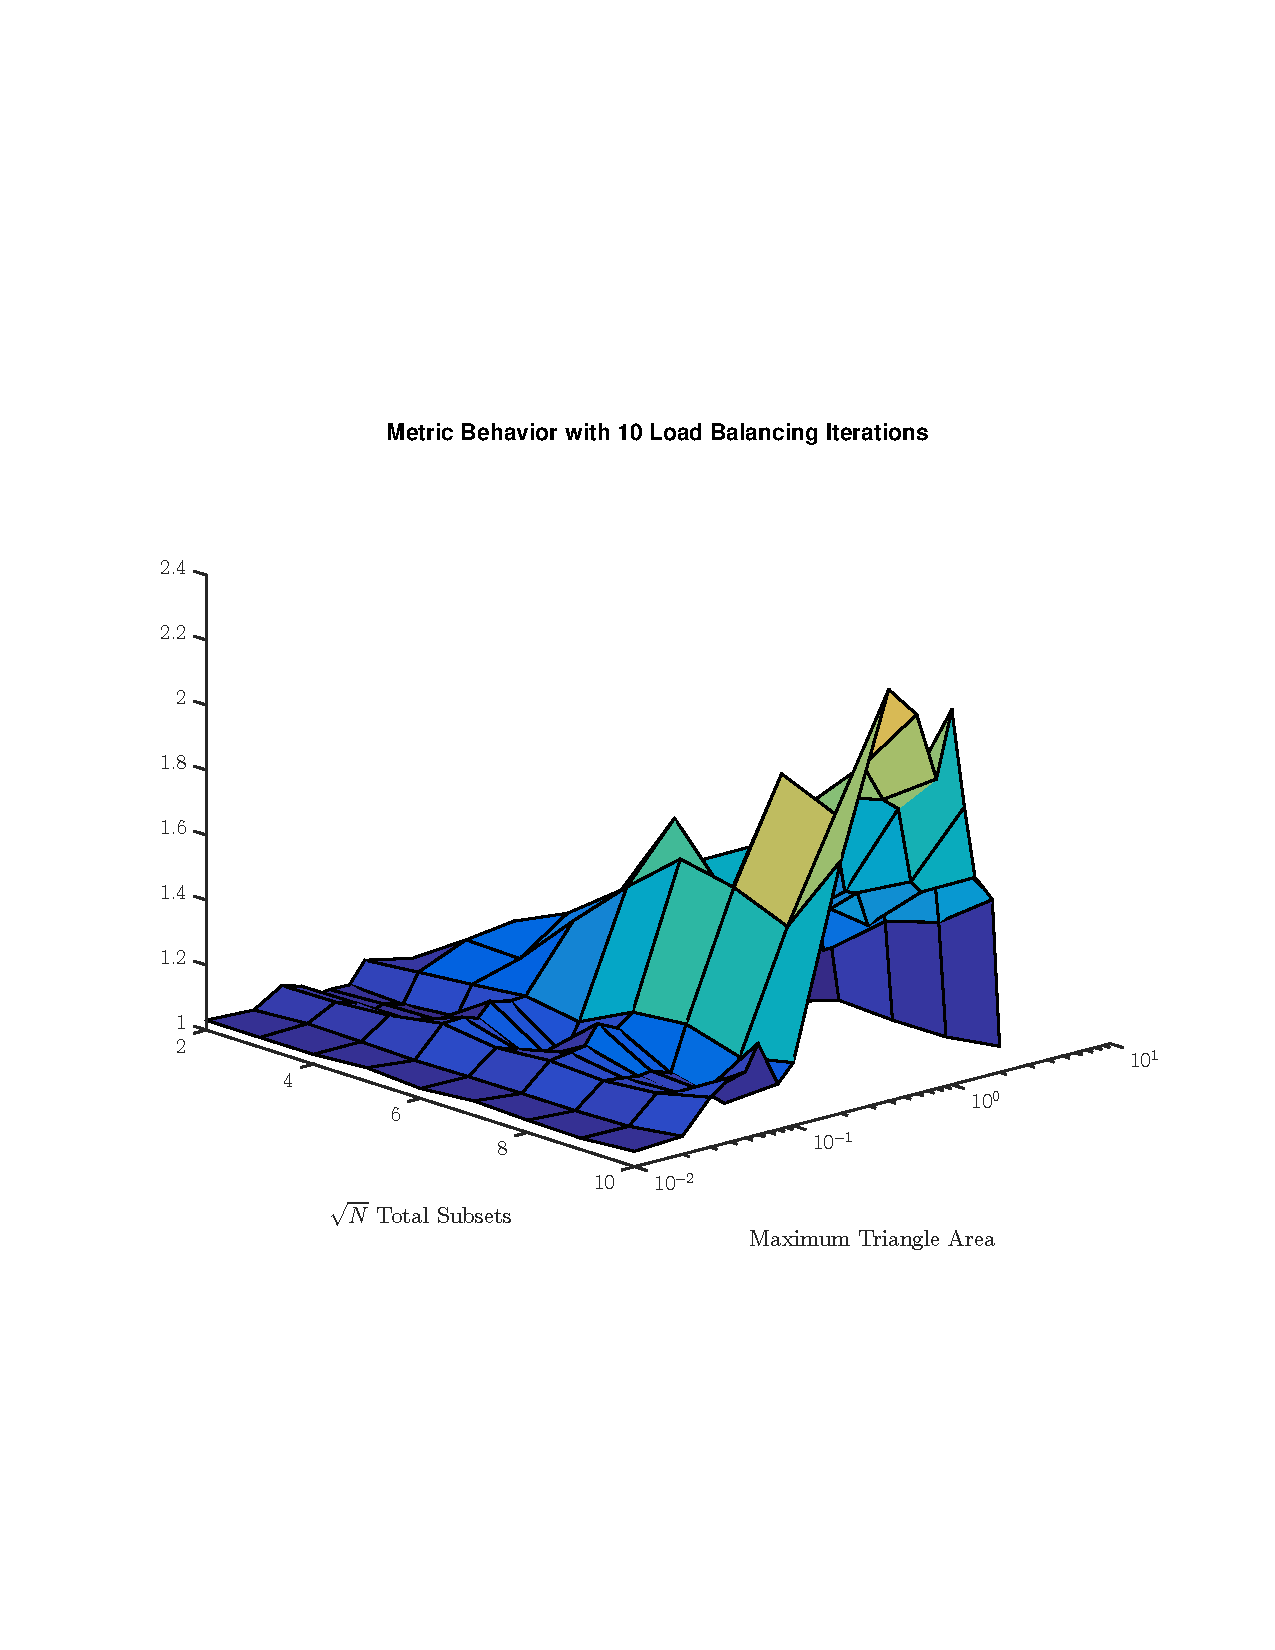
\includegraphics[scale=0.5, trim = 2cm 6cm 2cm 7cm,clip]{figures/lattice_iter.pdf}
\caption{The difference in metric behavior of the third test case after ten load balancing iterations.}
\label{latticeiter}
\end{figure}

Figure \ref{latticediff} shows the difference in metric behavior for Fig. \ref{lattice}. The maximum improvement has a value of 0.4476 and occurs for Fig. \ref{lattice} is run with 2x2 subsets with Triangle's coarsest possible mesh generation settings. The minimum improvement has a value of very close to 1.0 and occurs for many of the inputs. 

\begin{figure}[H]
\centering
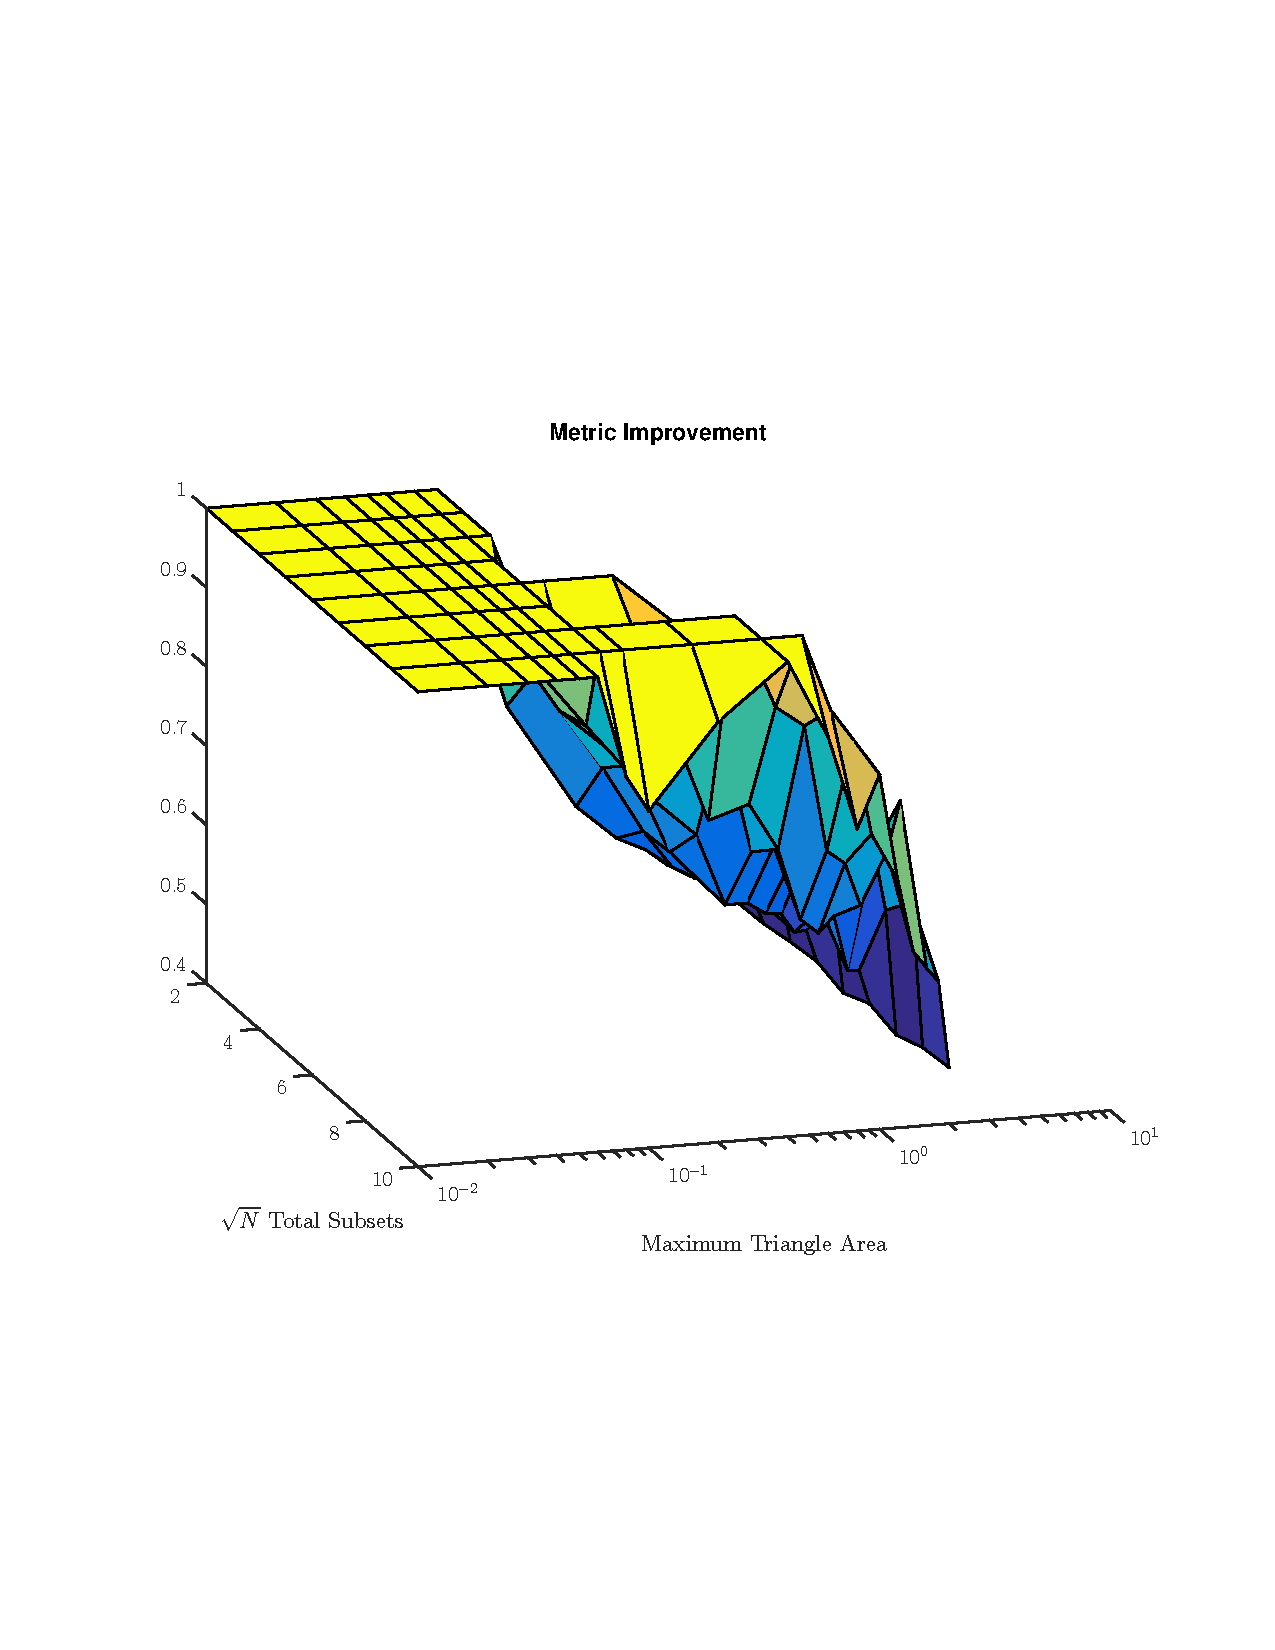
\includegraphics[scale=0.50, trim = 2cm 6cm 2cm 7cm,clip]{figures/lattice_diff.pdf}
\caption{The difference in metric behavior of the third test case with no iteration and 10 iterations. The closer the z-value to zero, the better the improvement.}
\label{latticediff}
\end{figure}

Because Fig. \ref{lattice} has more features and is more symmetric of a problem, the initial load balancing metric will not be as large as the load balancing metric of Figs. \ref{same} and \ref{opp}. As a result, the improvement in the load balancing metric after 10 iterations will not be as great in problems similar to Fig. \ref{lattice}. 

Good improvement is seen throughout all three test cases for all three inputs, particularly the first two test cases, which were initially very unbalanced. However, there were many inputs run that had problems with $f > 1.1$, which means many problems were unbalanced by more than 10\%. The user will not always have the luxury of choosing the number of subsets they want the problem run with, as this directly affects the number of processors the problem will be run with. Certain problems will require more processors and will require minimizing the total number of cells in the domain for the problem to complete running in a reasonable amount of time. As a result, improvements to the algorithm must be made. 

This can be done by changing how the cut lines are redistributed. Instead of changing entire row and column widths, the cut lines can be moved on the subset level. However, this can sacrifice the strict orthogonality that PDT currently utilizes to scale so well on a massively parallel scale. Changes to the performance model and the scheduler would have to be made.

Another option is to implement domain overloading, which is the logical extension of the work presented in this thesis. This would involve processors owning different numbers of subsets, with no restriction on these subsets being contiguous. This would be the most effective method at perfecting this algorithm, and would lead to less problems being unbalanced by more than 10\%.

\subsection{2D and 2D Extruded Meshing Capability}

To showcase, the newly implemented unstructured meshing capability in PDT, Texas A\&M Nuclear Engineering's Impurity Model 1 (IM1) problem is used. Figure \ref{IM12D} showcases the 2D mesh of the IM1 problem,

\begin{figure}[H]
\centering
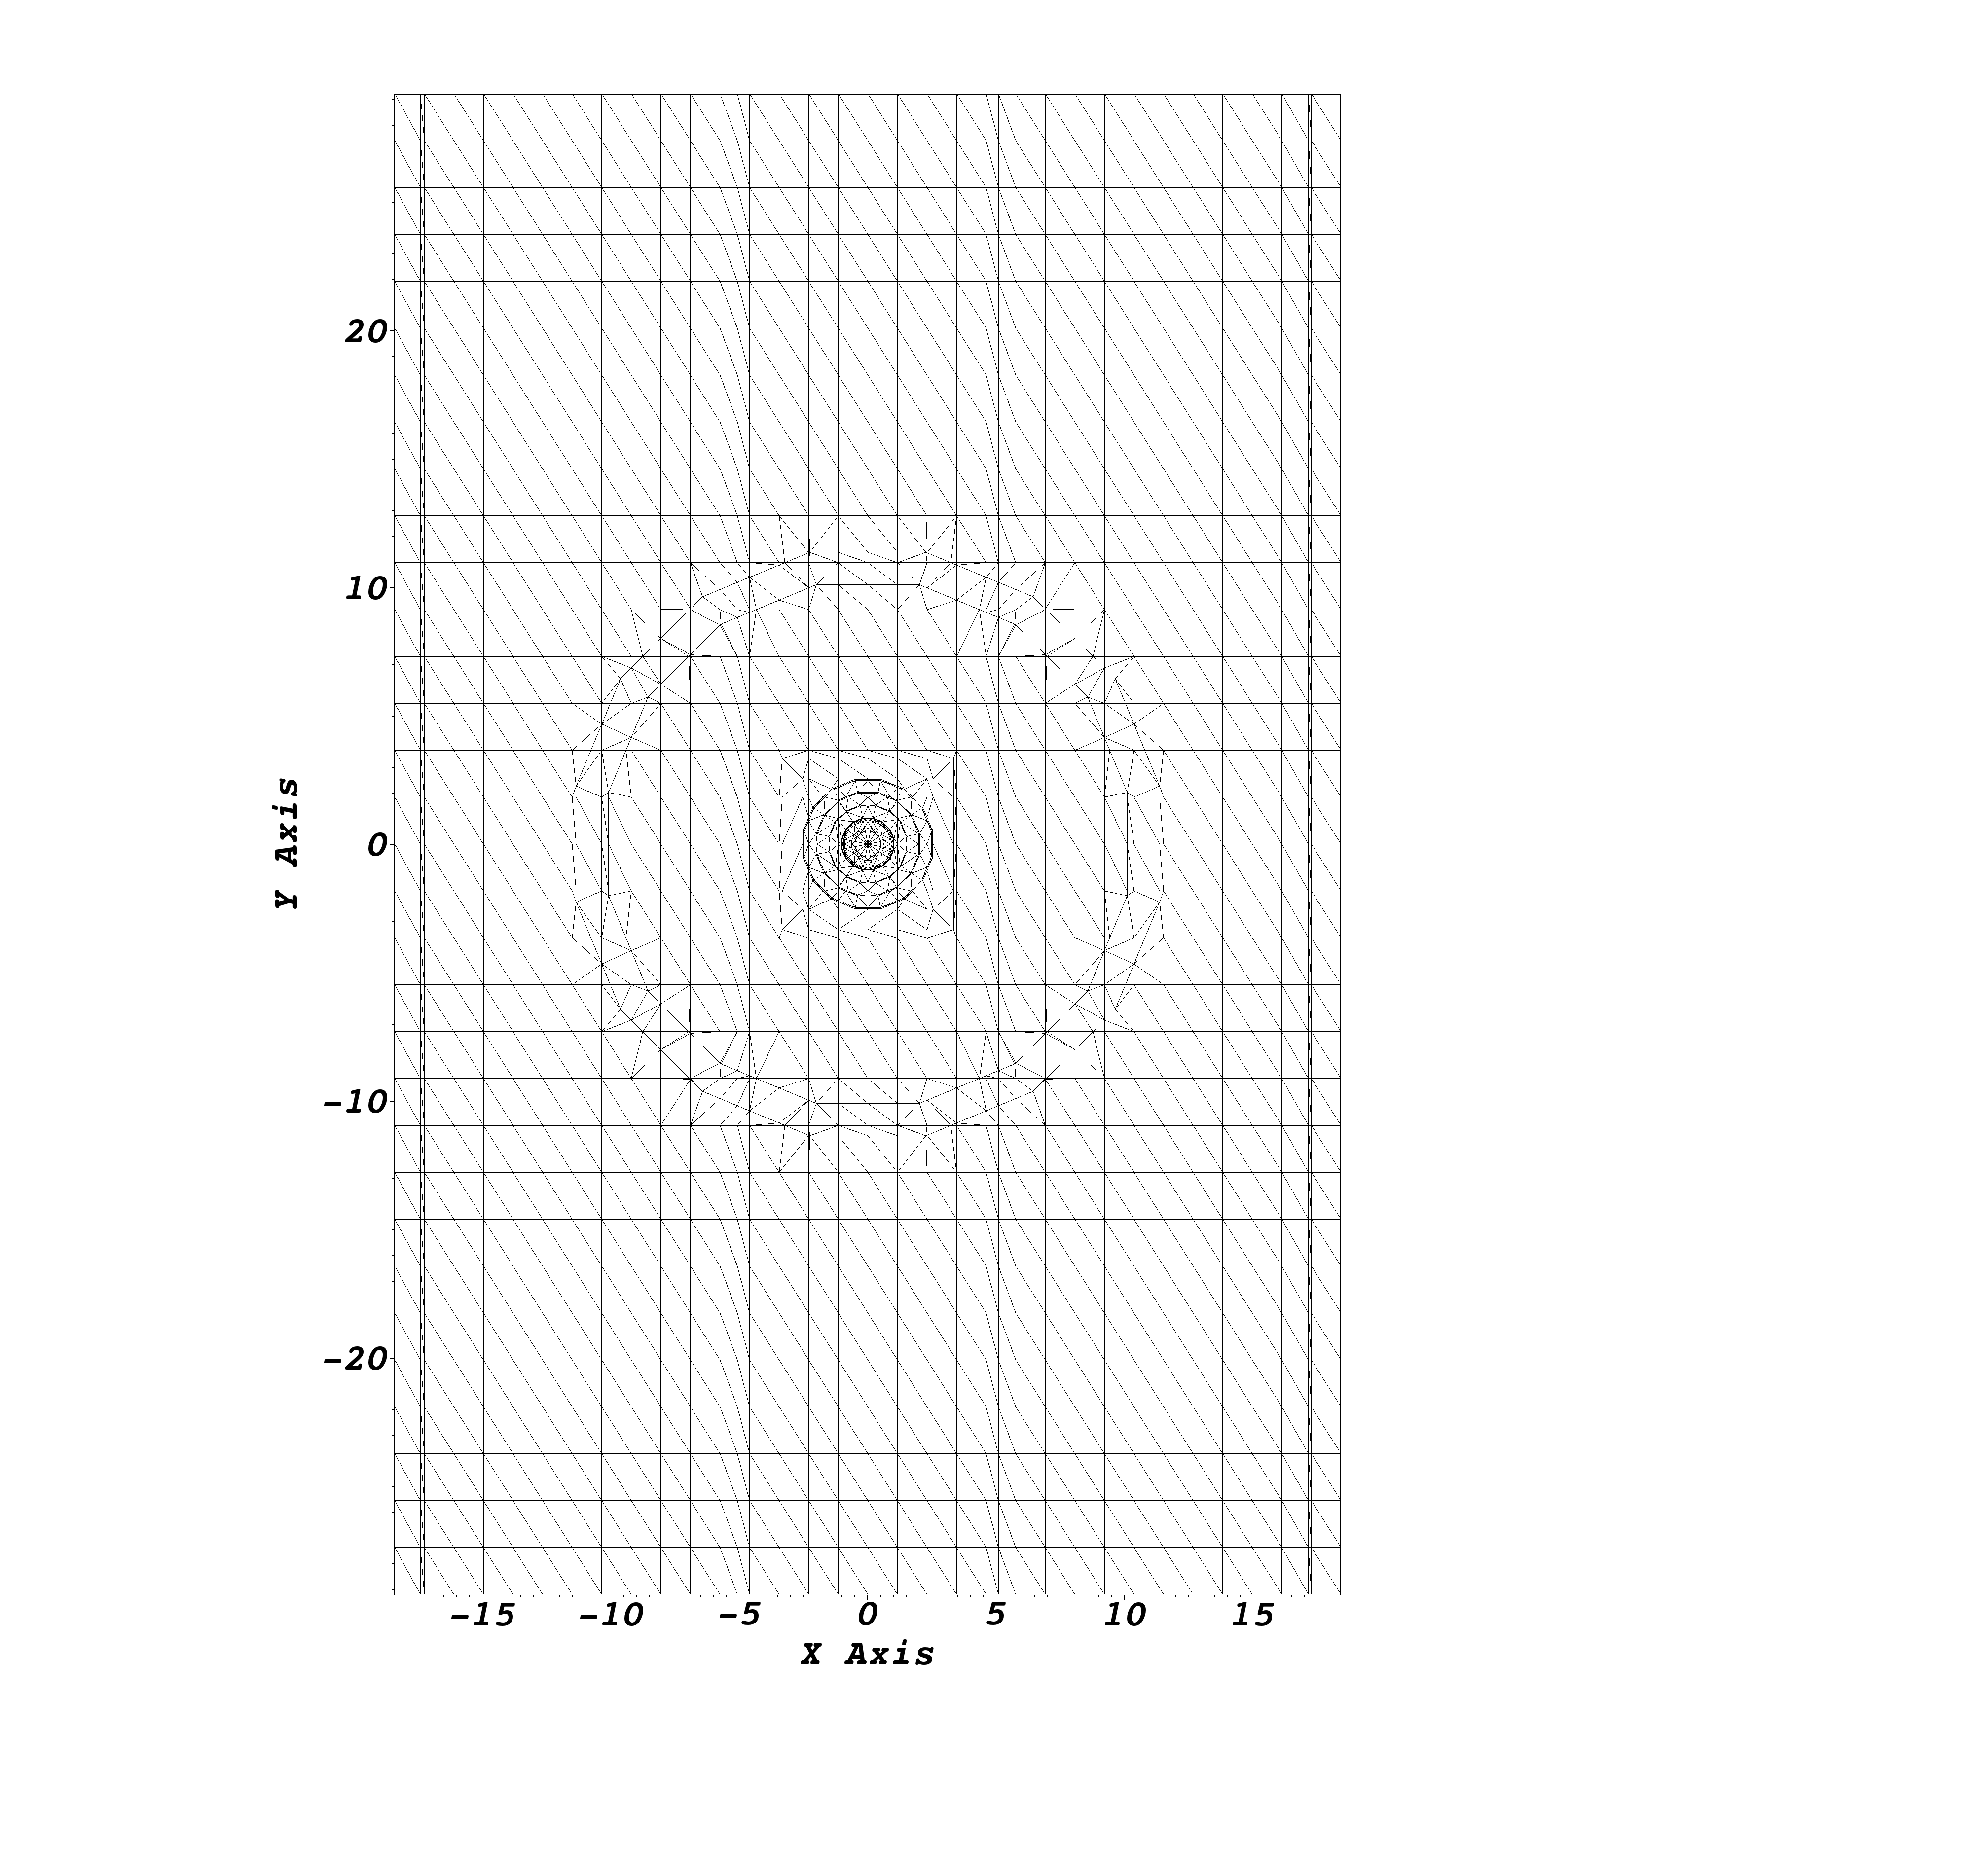
\includegraphics[scale = 0.13, trim=28cm  4cm 0cm 4cm,clip]{figures/im12d.png}
\caption{The 2D mesh of the IM1 problem.}
\label{IM12D}
\end{figure}

In order to get from the 2D mesh to the 2D extruded mesh, an extrusion file is supplied to PDT. This extrusion file supplies two critical pieces of information: the number of z layers and their locations, and how each region of the 2D mesh is mapped to these z layers. The combination of the 2D mesh and the extrusion file yield the full 3D problem, shown in Fig. \ref{IM13D}.

\begin{figure}[H]
\centering
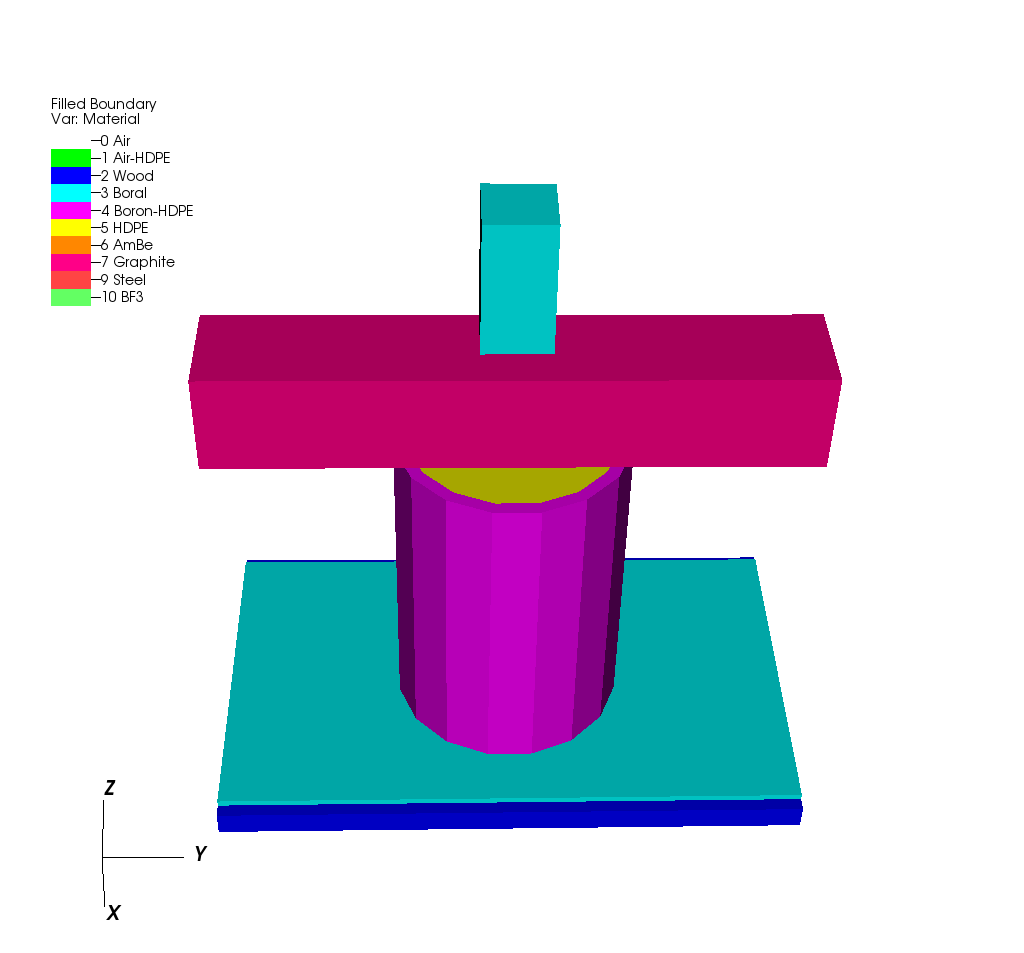
\includegraphics[scale = 0.3]{figures/IM1_3D.png}
\caption{The 2D extruded view of the IM1 problem.}
\label{IM13D}
\end{figure}

%%%%%%%%%%%%%%%%%%%%%%%%%%%%%%%%%%%%%%%%%%%%%%%%%%%%%%%%%%%%%%%%%%%%%%%%%%%%%%%%%%%%%%%%%%%%%%%%%%%%%%%%%%%%%%%%%%%%%%%%%%%%%%%%%%%%%%%%%%%
\section{Conclusions}

In conclusion, the load balancing algorithm outlined in the Motivation and Methods section works well for more symmetric problems with a lot of features, and even works well for particularly unbalanced problems. As shown in Chapter~\ref{ch:results}, its effectiveness depends on the maximum triangle area used, and the number of subsets the user chooses to decompose the problem domain into. 

Good improvement is seen throughout all three test cases for all three inputs, particularly the first two test cases, which were initially very unbalanced. However, there were many inputs run that had problems with $f > 1.1$, which means many problems were unbalanced by more than 10\%. The user will not always have the luxury of choosing the number of subsets they want the problem run with, as this directly affects the number of processors the problem will be run with. Certain problems will require more processors and will require minimizing the total number of cells in the domain for the problem to complete running in a reasonable amount of time. As a result, improvements to the algorithm must be made. 

This can be done by changing how the cut lines are redistributed. Instead of changing entire row and column widths, the cut lines can be moved on the subset level. However, this can sacrifice the strict orthogonality that PDT currently utilizes to scale so well on a massively parallel scale. Changes to the performance model and the scheduler would have to be made.

Another option is to implement domain overloading, which is the logical extension of the work presented in this thesis. This would involve processors owning different numbers of subsets, with no restriction on these subsets being contiguous. This would be the most effective method at perfecting this algorithm, and would lead to less problems being unbalanced by more than 10\%.

%%%%%%%%%%%%%%%%%%%%%%%%%%%%%%%%%%%%%%%%%%%%%%%%%%%%%%%%%%%%%%%%%%%%%%%%%%%%%%%%

%%%%%%%%%%%%%%%%%%%%%%%%%%%%%%%%%%%%%%%%%%%%%%%%%%%%%%%%%%%%%%%%%%%%%%%%%%%%%%%%
\section{Acknowledgments}
This material is based upon work supported a Department of Energy Nuclear
Energy University Programs Graduate Fellowship.

%%%%%%%%%%%%%%%%%%%%%%%%%%%%%%%%%%%%%%%%%%%%%%%%%%%%%%%%%%%%%%%%%%%%%%%%%%%%%%%%
\bibliographystyle{ans}
\bibliography{bibliography}
\end{document}

